\documentclass[conference]{IEEEtran}
\IEEEoverridecommandlockouts
% The preceding line is only needed to identify funding in the first footnote. If that is unneeded, please comment it out.
\usepackage{cite}
\usepackage{amsmath,amssymb,amsfonts}
\usepackage{algorithmic}
\usepackage{graphicx}
\usepackage{textcomp}
\usepackage{xcolor}
\usepackage[croatian]{babel}
\usepackage[T1]{fontenc}
\def\BibTeX{{\rm B\kern-.05em{\sc i\kern-.025em b}\kern-.08em
    T\kern-.1667em\lower.7ex\hbox{E}\kern-.125emX}}
\graphicspath{ {./images/} }
\begin{document}

\title{Metode za automatsku
ravnotežu boja (auto white balance)
}

\author{\IEEEauthorblockN{1\textsuperscript{st} Lana Šprajc}
\IEEEauthorblockA{\textit{Fakultet eletrotehnike i računarstva} \\
\textit{lana.sprajc@fer.hr} }
\and
\IEEEauthorblockN{2\textsuperscript{nd} Lara Grgurić}
\IEEEauthorblockA{\textit{Fakultet eletrotehnike i računarstva} \\
\textit{lara.grguric@fer.hr} }
\and
\IEEEauthorblockN{3\textsuperscript{rd} Maja Polanec}
\IEEEauthorblockA{\textit{Fakultet eletrotehnike i računarstva} \\
\textit{maja.polanec@fer.hr} }
\and
\IEEEauthorblockN{4\textsuperscript{th} Toni Polanec}
\IEEEauthorblockA{\textit{Fakultet eletrotehnike i računarstva} \\
\textit{toni.polanec@fer.hr} }
\and
\IEEEauthorblockN{5\textsuperscript{th} Milan Vrankić}
\IEEEauthorblockA{\textit{Fakultet eletrotehnike i računarstva} \\
\textit{milan.vrankic@fer.hr} }
}

\maketitle

\begin{abstract}
This document is a model and instructions for \LaTeX.
This and the IEEEtran.cls file define the components of your paper [title, text, heads, etc.]. *CRITICAL: Do Not Use Symbols, Special Characters, Footnotes, 
or Math in Paper Title or Abstract.
\end{abstract}

\begin{IEEEkeywords}
Hubble, astrofotografija, auto white, ravnoteža boja
\end{IEEEkeywords}

\section{Uvod}
Svemirski teleskop Hubble je program suradnje Europske svemirske agencije i
Nacionalne uprave za aeronautiku i svemir. Pojedinačne slike s Hubbleovih kamera
ne sadržavaju nikakvu informaciju o boji kao takvoj, osim boje filtra, koji
odabire niz valnih duljina iz cijelog spektra svjetlosti. Crno-bijela (jednobojna)
slika najrealističnije predstavlja raspon svjetline u takvoj jednoj slici. Usprkos
tomu, slike u boji mogu se rekonstruirati kombiniranjem nekoliko slika napravljenih
kroz različite filtre i dodjeljivanjem različite boje svakoj slici. Želimo testirati
metode balansiranja boja na astrofotografijama napravljenima koristeći
Svemirski teleskop Hubble.

\section{Pregled literature}
Vrijednost piksela ovisi o boji izvora, refleksiji površine i osjetljivosti kamere.
Budući da ovi parametri nisu poznati, potrebne su metode procjene parametara \cite{article}.

Jedna od skupina metoda procjene boje izvora su statičke metode. U njoj se primjenjuju
fiksni parametri nad ulaznom slikom. Najkorištenija statička metoda je pretpostavka sivog
svijeta (engl. \textit{Grey-World Assumption}). Početna pretpostavka ove metode jest da je
prosječna refleksija površine siva te se zaključuje da ukupna prosječna boja u slici proizlazi
iz izvora. Tako se pojedina RGB komponenta izvora računa kao integral te komponent kroz
cijelu sliku pomnožen s nekim skalarom (kako bi se izvor normirao) \cite{BUCHSBAUM19801}.

Druga skupina često korištenih metoda procjene boje su metode bazirane na gamutu.
Osnovna pretpostavka ove metode je da za dani izvor svjetlosti možemo primjetiti
samo ograničeni skup boja. U fazi treniranja ove metode određuje se koji skup boja
možemo očitati za određene izvore. Nakon treniranja, za ulaznu sliku odredi se skup
boja koje ona sadržava te se definira koji su mogući izvori svjetlosti za taj skup boja.
Nakon toga se odabire neki od mogućih izvora svjetlosti i primjenjuje se tranformacija nad
slikom kako bi se dobila balansirana slika \cite{Forsyth1990}.


\section{Opis rješenja}

Slike su dane u .fits formatu. Fits je format otvorenog standarda koji se koristi u prijenosu fotografija s teleskopa. Budući da se različiti tipovi podataka mogu prenositi u tom formatu, sama slika je formatirana kao 2D polje gdje svaki element polja predstavlja intenzitet točke. Promatramo 2 tipa fotografija (reprezentiranih kao 2D polje), a to su UVIS (Ultraviolet Imaging Spectrograph) i IR (Infrared) fotografije. Budući da slike ne nose informaciju o boji to je potrebno primijeniti. Naime, teleskop slika prikazuje na različitim valnim duljinama elemente kao što su kisik, vodik i sumpor. Valna duljina dvo dimenzionalnog polja je dana u samom opisu datoteke. Uz navedeno dane su i informacije o tipu korištenog senzora i informacija je li polje težina ili "drizzled image". Pri izradi koristimo biblioteku Astropy za Python3. Prvo ćemo učitati matrice iz fits slika, te osigurati da sve NaN vrijednosti stavimo na 0 (ove vrijednosti se pojavljuju zbog mikro oštećenja na senzoru i radijacije). No, ne možemo još složiti našu sliku. Primijetimo da valne duljine koje smo dobili odgovaraju crvenoj boji, zbog čega? Prisjetimo se da pad frekvencije odgovara "red shiftu" jer se objekti koje snimamo udaljavaju od nas, no i dalje se vide razlike u valnim duljinama. Ono što nam ostaje je mapirati te valne duljine na crvenu, plavu i zelenu. Ako smo dobili 3 datoteke od kojih jedna odgovara 502nm (plava boja), te druge dvije 657nm (crvena boja) i 673nm (crvena boja). Ono što ćemo uraditi je to da ćemo uzeti sliku od 657nm i spustiti ju u područje ispod 600nm. No ni to ne daje najbolje rezultate jer smo umjetno mijenjali jednu valnu duljinu a da smo ostale valne duljine ostavili na svom mjestu. Iz tog razloga smo tražili 99 percentil svakog kanala te maksimalni intenzitet točke (koji je 256) podijelili s tim brojem. Time smo dobili omjere koje ćemo množiti s originalnim vrijednostima intenziteta točke te ih fiksirati u omjer od 0 do 256. Tim smo balansirali sve kanale matrice, no ni dalje ne izgleda jako lijepo. Ono što možemo pokušati je promijeniti krivulju boje. Uzet ćemo model linearne regresije naučen na svojoj boji, kojoj su ciljne vrijednosti ostale boje. Ona točna boja će odgovarati aritmetičkoj sredini npr. modela crvene boje s ciljnim vrijednostima zelene boje i modela crvene boje s ciljnim vrijednostima plave boje. Nakon što te vrijednosti ubacimo u interval od 0 do 256 dobivamo balansirane krivulje boja. Sljedeći korak je smanjiti šum slike, za to ćemo koristiti "Non-Local Means Denoising" algoritam koji je ugrađen u paket cv2. Na kraju ako želimo da slika bude oku ugodnija možemo promijeniti svjetlinu i živost slike. Prvo ćemo sliku pretvoriti iz rgb u hsv sustav. Nakon toga množiti v i s vrijednosti s konstantama koje se nama osobno više sviđaju (ova procedura je empirijska te se gube detalji). Što se tiče infracrvenih slika tu dobivamo 2 slike, obično jedna slika predstavlja plavi kanal dok druga predstavlja žutu ili narančastu boju, te je potrebno odvojiti taj kanal u 2 umjetna kanala, te ponoviti proceduru kao i za uvis slike.

\section{Opis eksperimentalnih rezultata}

Kao što je prije navedeno, slike su izvorno u .fits formatu. Taj format nije najbolji za direktni prikaz. Slike su gotovo cijele bijele ili crne s sitnim kontrastnim točkicama. Prikaz svih 3 .fits izvornih slika vidimo na Slici 1.
\begin{figure}[h]
    \centering
    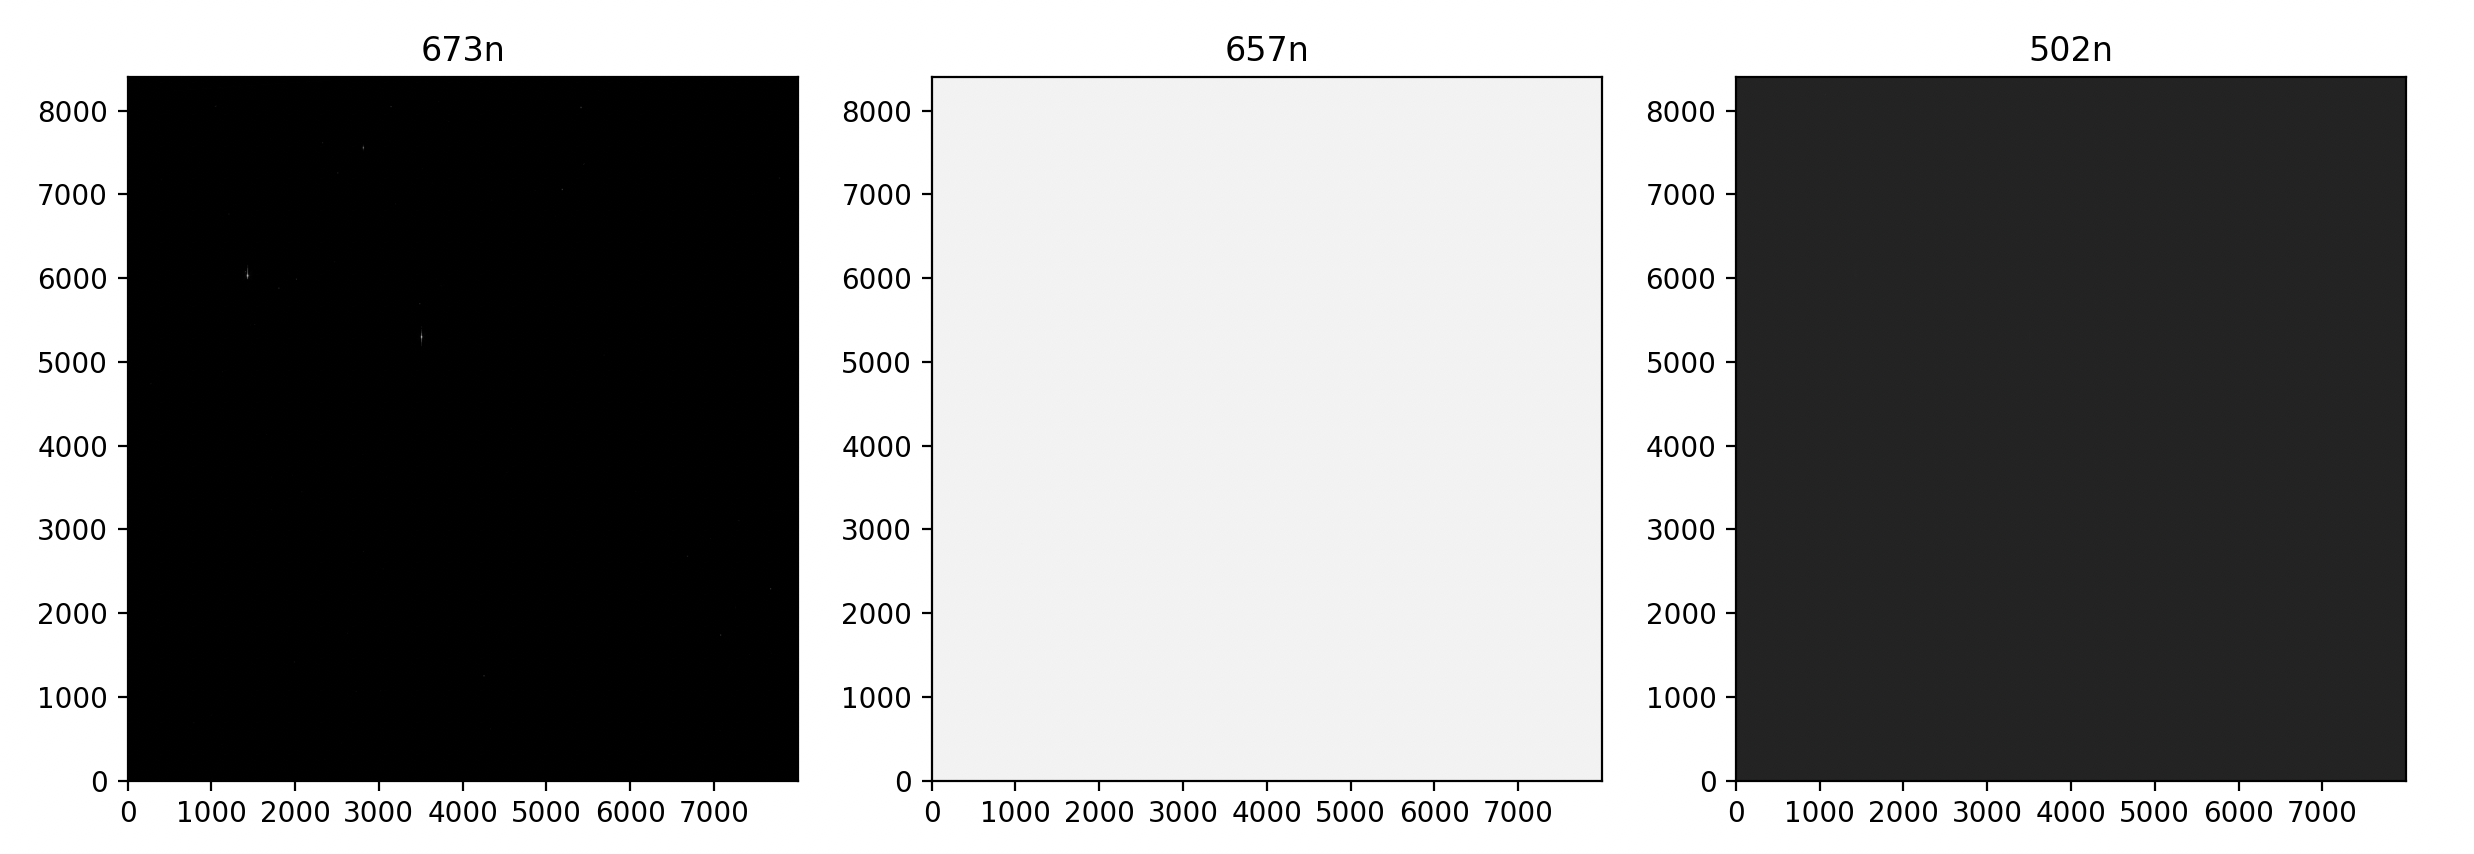
\includegraphics[width=0.5\textwidth]{specks}
    \caption{Prikaz .fits formata}
    \label{slika:s1}
\end{figure}

Njihovim spajanjem i specifičnim alteriranjem pojedinih valnih duljina i balansiranjem možemo dobiti sliku koja je nama puno više pogodna za prikaz i zapravo pregled toga što smo fotografirali teleskopom. Prikaz Eagle nebule poznate pod imenom "Pillars of Creation" možemo vidjeti na slici 2.
\begin{figure}[h]
    \centering
    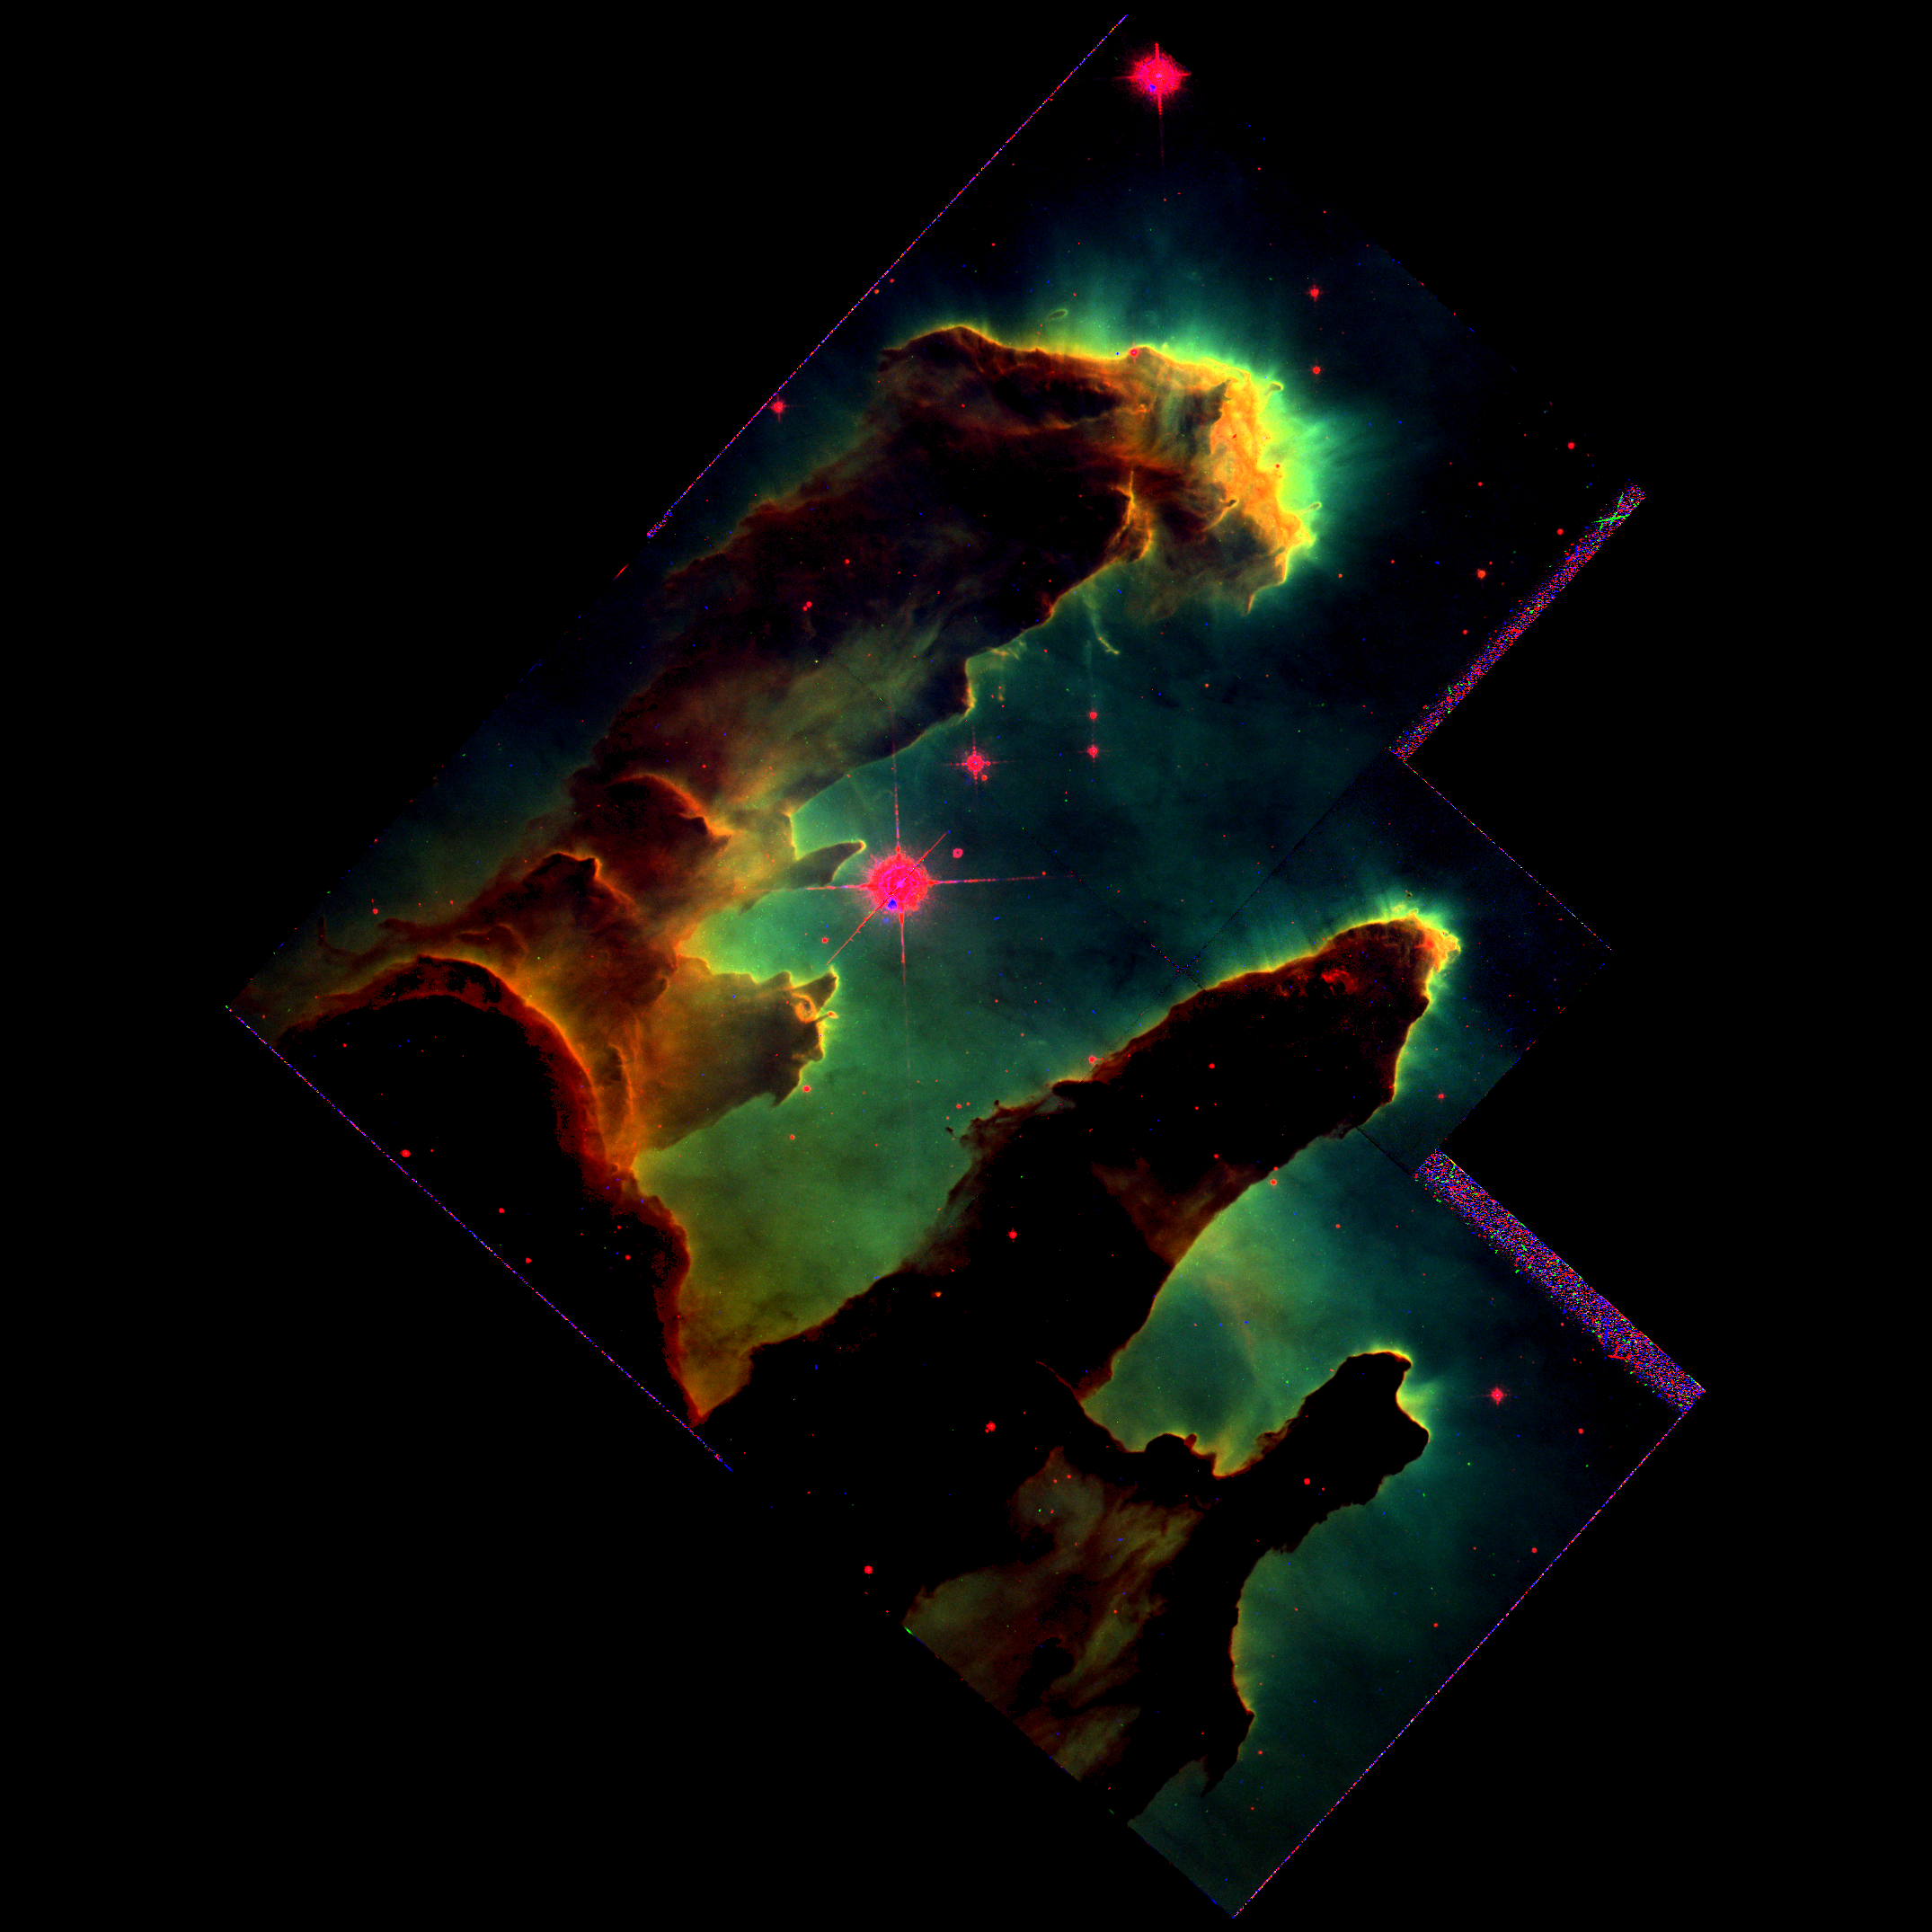
\includegraphics[width=0.45\textwidth]{pillar}
    \caption{Eagle nebula}
    \label{slika:s2}
\end{figure}

Bitna stavka procesiranja slika je uklanjanje ili smanjivanje šuma u slici. Funkcija 
\begin{verbatim}
    cv2.fastNlMeansDenoising()
\end{verbatim}
koja implementira Non-Local Means Denoising algoritam nam je prikladna zbog načina uklanjanja šuma. Naime, u našim slikama šum će se najčešće pojaviti kao smetnja u procesu fotografiranja u obliku nasumičnih piksela koji odudaraju od ostatka slike. Navedeni algoritam, tj. metoda uklanjanja šuma radi na način da za pojedini piksel uzme prozorčić oko njega i pronađe slične prozorčiće u ostatku slike. Uprosječuje sve slične prozorčiće i postavlja vrijednost piksela na tu uprosječenu vrijednost \cite{fastNlMeansDenoising}. Kod našeg se problema ta metoda pokazala jako uspješnom.

Razlika dijela slike sa šumom i dijela slike sa smanjenim šumom može se primijetiti na slici 4.
\begin{figure}[h]
    \centering
    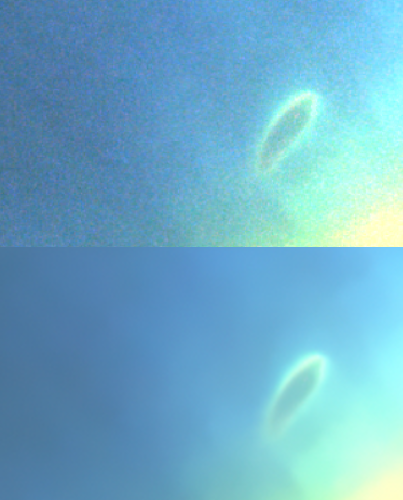
\includegraphics[width=0.45\textwidth]{noise_denoised}
    \caption{Prikaz djelovanja algoritma uklanjanja šuma}
    \label{slika:s4}
\end{figure}


"Fotografiranjem" infracrvenim zrakama dobijemo 2 slike (Slika 4). Jedna većinski plava, druga pak ima žućkastu nijansu. Njihovim spajanjem (koje se svodi na ručno ugađanje parametara) dobivamo sve RGB kanale i možemo je prikazati u boji na slici 5. Balansiranje i smanjivanje šuma napravljeno je istovjetno prijašnjem primjeru.
\begin{figure}[h]
    \centering
    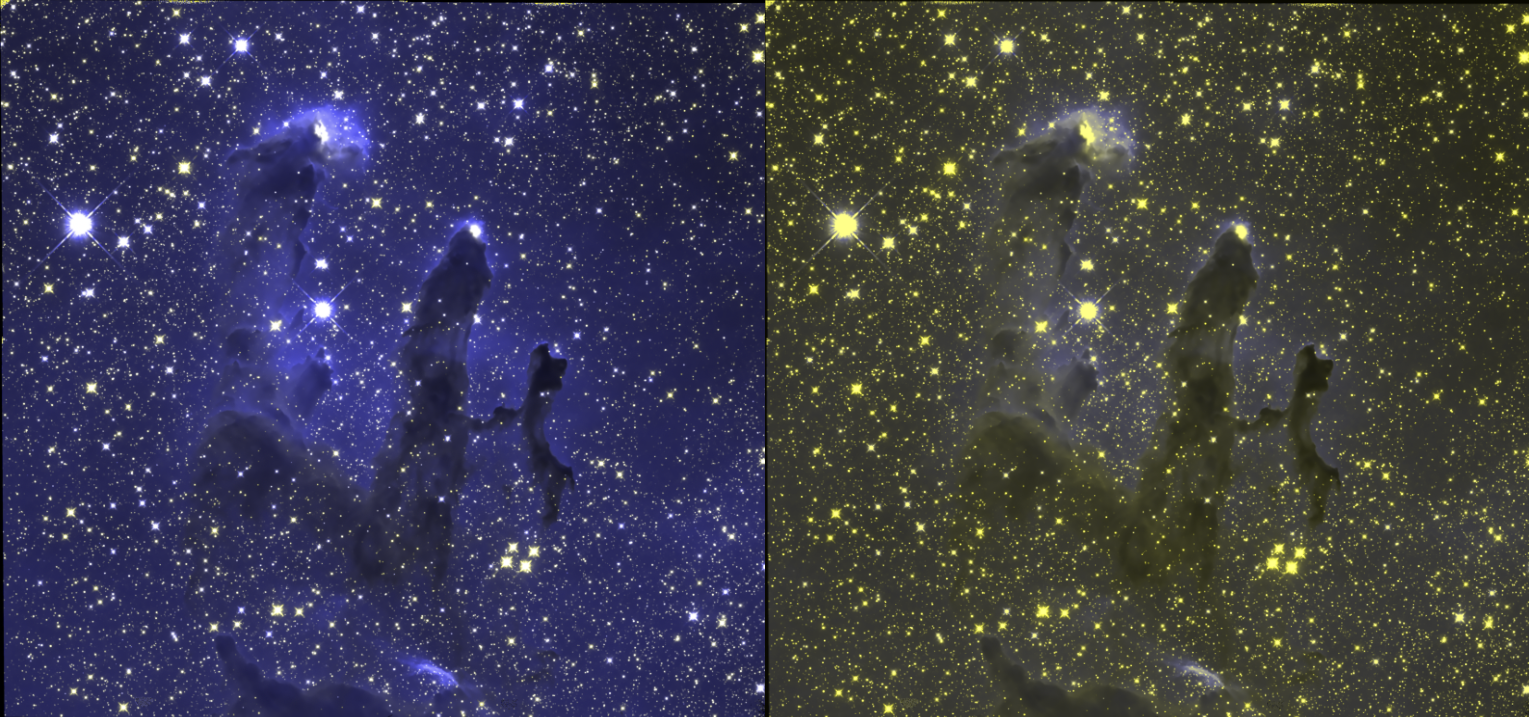
\includegraphics[width=0.5\textwidth]{IC_kanali}
    \caption{Slike dobivene IC fotografiranjem}
    \label{slika:s5}
\end{figure}
\begin{figure}[h]
    \centering
    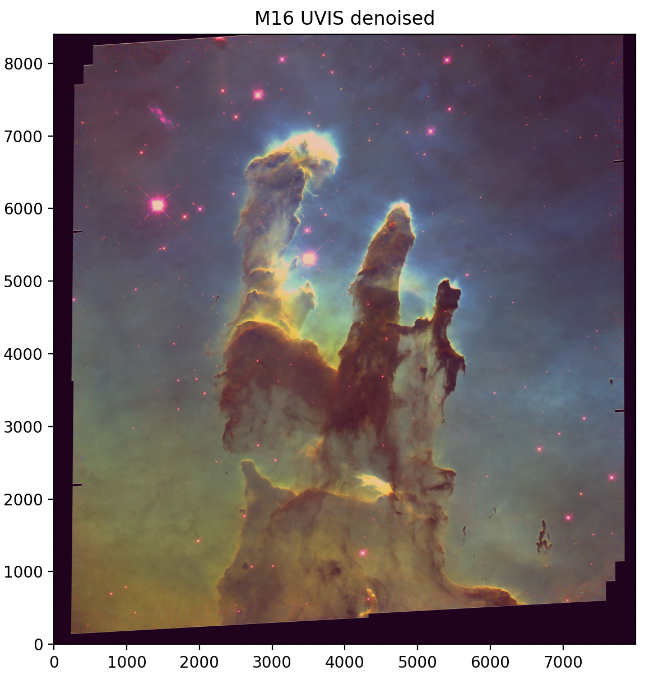
\includegraphics[width=0.45\textwidth]{IC_colorized}
    \caption{Obojana IC slika}
    \label{slika:s5}
\end{figure}

\section{Diskusija}

Moramo biti svjesni da ovdje baratamo sa \textit{false colorom}. Kada nam teleskop izbaci skenove određenih valnih duljina mi si ih prilagođavamo i prikazujemo na onaj način koji nama najviše paše. Npr. volimo vidjeti kontrastne slike i one su i u istraživanjima korisne jer se vide detaljne razlike u slikama. Isto tako, kada čovjek zamisli svemir, umjesto realne slike tame i crne beskonačnosti zamišljamo šarene nebule, eksplozije zvijezda i svakojake crvotočine (sci-fi filmovi su najviše pomogli ovdje). Prema tim očekivanjima se i ugađaju na prvu, besmislene slike. Jasno je tada da je cilj prilagodbe početnih beznačajnih slika dobiti šarene slike visokog kontrasta.

Prikaz rezultata algoritma pretpostavke sivog svijeta (engl. \textit{Gray world assumption}) je na slici 6. Na lijevoj strani je naš rezultat, a na desnoj strani je rezultat sivog svijeta. Ne vidi se prevelika razlika. Najvidljivije je to što se slika malo posvijetlila. Algoritam nema smisao u našem problemu jer pokušavamo dobiti kontrastne slike.
\begin{figure}[h]
    \centering
    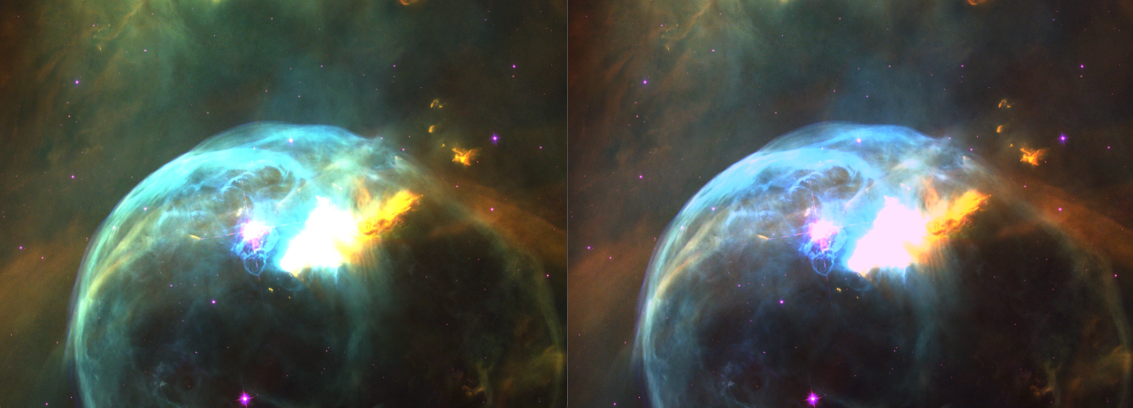
\includegraphics[width=0.45\textwidth]{greyworld}
    \caption{Rezultat pretpostavke sivog svijeta}
    \label{slika:s5}
\end{figure}

Neki drugi algoritmi poput \textit{White Patch Algorithm} (na temelju bijele boje u RGB formatu (255,255,255) skalira kanale boja i s time dobije svjetliju/više bijelu sliku) ili \textit{Ground-Truth Algorithm} (ručno odabiremo dio slike koji znamo da je točan, npr. snijeg je potpuno bijel te prema tome balansiramo ostatak slike \cite{Nigam2021}) nemaju smisla u astrofotografijama jer nemamo cilj prema kojem gravitiramo. Npr. kod \textit{Ground-Truth Algorithm} znamo da je snijeg bijeli i uz pomoć tog popravljamo sliku. Kod astrofotografije nemamo dio slike koji znamo da je npr. zelen i većina algoritama (koji su primarno tu zbog balansiranja svakodnevnih slika) nemaju smisla jer ne možemo na isti način popravljati slike nebula, svemirskih maglica i ostale svemirske pojave.



\section{Zaključak}

\listoffigures
\bibliographystyle{IEEEtran}
\bibliography{IEEEfull}
\vspace{12pt}

\end{document}
